\chapter{\textit{Android}}

\section{Sejarah \textit{Android}}
Android merupakan sistem operasi berbasis linux yang dirancang untuk perangkat bergerak atau layar sentuh seperti \textit{smartphone} dan \textit{tablet}. Android adalah sistem operasi dengan sumber terbuka, dan Google merilis kodenya di bawah Lisensi Apache. Lisensi Apache adalah sebuah lisensi perangkat lunak-bebas yang ditulis oleh Apache Software Foundation (ASF). Android didirikan di Palo Alto, California pada bulan Oktober tahun 1980 oleh Andy Rubin, Rich Muner, Nick Sears, dan Chris White. Awalnya android dikembangkan oleh perusahaan yang bernama \textit{Android, Inc} yang mendapat dukungan finansial dari \textit{Google}, yang kemudian dibeli oleh \textit{Google} pada tahun 2005. Android awalnya tidak dibuat untuk ponsel, melainkan android dibuat untuk kamera digital. Karena peluang pada perangkat mobile lebih besar untuk berkembangjadi Android diplot untuk menyaingi Symbian dan Windows Mobile.

Android secara resmi dirilis pada tahun 2007 bersamaan dengan didirikannya \textit{Open Handset Alliance}. \textit{Open Handset Alliance} adalah pengembangan standar terbuka bagi perangkat selular. Pada tahun 2008 HP pertama yang menggunakan sistem operasi android akhirnya dirilis, yaitu HTC Dream. Dua tahun berselang, Google melepaskan ponsel pintar seri Nexus One yang proses pembuatannya dibantu oleh HTC. Kemudian muncul berbagai brand dari OEM yang berbeda mulai dari Samsung, LG, Asus, Lenovo, HTC, dan lain sebagainya. Selain pada \textit{smartphone}, Google juga mengembangkan Android TV untuk televisi, Android Auto untuk mobil, dan Android Wear untuk jam tangan, yang masing-masing memiliki interface yang berbeda. Kode dengan sumber terbuka dan lisensi perizinan pada Android memungkinkan perangkat lunak untuk dimodifikasi secara bebas dan didistribusikan oleh para pembuat perangkat, operator nirkabel, dan pengembang aplikasi. Selain itu, Android memiliki sejumlah besar komunitas pengembang aplikasi (apps) yang memperluas fungsionalitas perangkat, umumnya ditulis dalam versi kustomisasi bahasa pemrograman Java. Pada bulan Oktober 2013, ada lebih dari satu juta aplikasi yang tersedia untuk Android, dan sekitar 50 miliar aplikasi telah diunduh dari Google Play, toko aplikasi utama Android.

Sejak tahun 2008, Android secara bertahap telah melakukan sejumlah pembaruan untuk meningkatkan kinerja sistem operasi, menambahkan fitur baru, dan memperbaiki bug yang terdapat pada versi sebelumnya. Setiap versi utama yang dirilis dinamakan secara alfabetis berdasarkan nama-nama makanan pencuci mulut atau camilan bergula; misalnya, versi 1.5 bernama Cupcake, yang kemudian diikuti oleh versi 1.6 Donut. Versi terbaru adalah 9.0 Pie, yang dirilis pada 7 maret 2018

\section{Versi Pada Android}
Sejak awal dipublikasikan, Android telah mempunyai banyak versi. Berbagai versi android dengan fitur-fitur keunggulannya masing-masing. Hal ini tentu disamping dengan pesaingnya yang sudah lama eksis, seperti Apple iOS, Windows, Blackberry (BB), Symbian dan sebagainya. Uniknya, setiap versi Android yang baru diluncurkan pasti selalu disertai dengan nama lucu yang sama sekali tidak ada hubungannya dengan karakter robot hijau (Android) tersebut.

\begin{enumerate}

\item Android 1.0 \textbf{Apple Pie}\\
Android versi pertama yaitu Apple Pie, yang dirilis pada 23 September 2008 dan hanya dilengkapi berbagai fitur seperti Play Store, kamera, Web Browser, Sinkronisasi antara G-mail, Contacts dan Google Agenda. Selain itu, diawal peluncurannya, Android juga sudah dilengkapi aplikasi Google Maps dan dukungan streaming Youtube. Google dan OHA merilis setidaknya ada 2 versi sebelum Android beta dirilis pada November 2007. Versi Alpha memiliki codename yaitu : Astro Boy, Bender dan R2-D2.

KELEBIHAN
Android Market, untuk mengunduh dan memperbarui aplikasi melalui toko aplikasi resmi Android.
Penjelajah web, untuk menampilkan, memperbesar dan melihat dalam layar penuh halaman web HTML dan XHTML.
Dukungan kamera, versi ini tidak memiliki pilihan untuk mengubah resolusi kamera, kejernihan, kualitas foto, dan sebagainya.
Memungkinkan pengelompokan sejumlah ikon aplikasi ke dalam satu folder di layar depan (homescreen).
Akses ke server surel web, mendukung POP3, IMAP4, dan SMTP
Sinkronisasi Gmail dengan aplikasi Gmail.
Sinkronisasi Google Contacts dengan aplikasi People
Sinkronisasi Google Calendar dengan aplikasi Calendar
Google Maps, dengan Latitude dan Street View untuk melihat peta dan citra satelit, serta menemukan lokasi bisnis dan petunjuk arah mengemudi dengan menggunakan GPS.
Google Sync, memungkinkan pengelolaan sinkronisasi pada aplikasi Gmail, People, dan Calendar.
Google Search, memungkinkan pengguna untuk mencari sesuatu di Internet.
Google Talk, aplikasi pesan instan.
Pesan instan, pesan teks (SMS), dan MMS.
Pemutar media, untuk mengelola, mengimpor, dan memutar berkas media, namun versi ini tidak menyediakan dukungan video dan Bluetooth stereo.[18][19]
Notifikasi muncul pada status bar, dengan pilihan untuk mengatur nada dering, LED, atau nada getar.[17][18][21]
Voice Dialer, memungkinkan pengguna untuk memanggil kontak tanpa harus mengetik nama atau nomor telepon.[18]
Wallpaper, memungkinkan pengguna untuk mengatur gambar latar belakang di layar depan.
Pemutar video YouTube.[22]
Aplikasi lainnya seperti: Jam Alarm, Kalkulator, Panggilan, Home screen (Launcher), Galeri, dan Pengaturan.
Dukungan Wi-Fi dan Bluetooth.

KEKURANGAN
versi ini android belum memiliki nama sehinggan masih belum mudah diingat masyarakat.


\item Android 1.1 \textbf{Banana Bread}\\
Sistem Operasi android yang rilis selanjutnya yaitu Banana Bread, rilis pada bulan Februari 2009. Dan fiturnya yaitu tidak jauh berbeda dengan versi sebelumnya. HTC merupakan salah satu smartphone Android pertama yang menggunakan versi ini. Android 1.1 juga dikenal dengan “Petit Four“, meskipun nama ini tidak digunakan secara resmi.[23] Versi ini memperbaiki beberapa bug, mengubah API Android, dan menambahkan beberapa fitur:
Rincian dan tinjauan tersedia saat pengguna mencari lokasi bisnis pada Peta.
Kemampuan untuk menampilkan/meenyembunyikan tombol panggilan.
Kemampuan untuk menyimpan lampiran pada pesan.
Menambah dukungan marquee pada tata ruang sistem.



\item Android 1.5 \textbf{Cupcake}\\
Dirilis pada awal bulan April 2009 dan juga tidak berbeda dengan versi Android sebelumnya. Hanya saja terdapat fitur tambahan seperti sudah Support Bluetooth A2DP, AVRCP, Soft-keyboard dengan prediksi text dan record atau watch videos. ersi ini adalah rilis pertama yang secara resmi menggunakan nama kode berdasarkan nama-nama makanan pencuci mulut (“Cupcake”), nama yang kemudian digunakan untuk semua versi rilis selanjutnya. Pembaruan pada versi ini termasuk beberapa fitur baru dan perubahan UI:
Dukungan papan ketik virtual pihak ketiga dengan prediksi teks dan kamus pengguna
Dukungan Widget – tampilan aplikasi miniatur yang tertanam dalam aplikasi lain dan menerima pembaruan secara periodik
Kemampuan merekam dan memutar video berformat MPEG-4 dan 3GP
Kemampuan memasangkan (pairing) dan dukungan stereo bagi Bluetooth (A2DP dan AVRCP)
Fitur salin dan tempel pada penjelajah web
Foto pengguna ditampilkan pada kontak favorit
Tanggal/waktu ditampilkan pada log panggilan, dan akses satu sentuhan ke nomor kontak dari log panggilan
Transisi layar animasi
Opsi memutar-otomatis
Animasi boot baru
Kemampuan untuk mengunggah video ke YouTube
Kemampuan untuk mengunggah foto ke Picasa



\item Android 1.6 \textbf{Donut}\\
Android Donut dirilis pada 15 September 2009, dan terdapat fitur tambahan seperti Gesture Framework hingga Turn-by-turn navigation. Kemudian, Android ini juga terlihat lebih sempurna pada saat itu. Dengan minimnya bug, ditambah lebih lengkapnya berbagai fitur yang disediakan oleh Google. Fitur-fitur barunya adalah sebagai berikut:
Entri pencarian teks dan suara diperluas, termasuk menyertakan riwayat bookmark, kontak, dan web
Kemampuan bagi para pengembang untuk menyertakan konten mereka pada hasil pencarian
Mesin sintesis pengucapan multibahasa yang memungkinkan aplikasi Android tertentu mampu mengucapkan teks
Pencarian yang lebih mudah dan kemampuan untuk melihat cuplikan aplikasi di Android Market
Galeri, kamera, dan perekam video yang lebih terintegrasi, dengan akses kamera yang lebih cepat
Kemampuan memilih banyak foto untuk dihapus
Pembaruan dukungan teknologi bagi CDMA/EVDO, 802.1x, VPN, dan mesin pengucap teks
Dukungan bagi resolusi layar WVGA
Peningkatan kecepatan dalam pencarian dan aplikasi kamera
Perluasan kerangka kerja Gestur dan penambahan perkakas pengembangan GestureBuilder.

KEKURANGAN
Tidak semua aplikasi (.apk) bisa di install di sini.
Music playernya belum ada equalizernya.
Android market yang tidak integrated
Keypad nya lemot dan touch responsiveness nya kurang sip daripada versi sesudahnya



\item Android 2.0 \textbf{Eclair} (API level 5)\\
Android versi 2.0 ini bernama Eclair dan dirilis pada 26 Oktober 2009 silam. Selain terdapat bluetooth, versi ini juga mendapatkan fitur tambahan seperti multi-touch, Live Wallpaper dan juga flash kamera. Kemudian, beberapa fitur yang dapat anda nikmati dalam versi eclair adalah HTML, Digital zoom, Support Microsoft Exchange, dan Updated UI. Perubahan pada versi ini meliputi:
Sinkronisasi akun diperluas, yang memungkinkan pengguna menambahkan beberapa akun untuk sinkronisasi surel dan kontak
Dukungan surel Microsoft Exchange, dengan kemampuan menjelajah surel dari beberapa akun dalam satu halaman
Dukungan Bluetooth 2.1
Kemampuan untuk memilih foto kontak dan opsi untuk memanggil, mengirim SMS atau surel kepada kontak yang bersangkutan
Kemampuan untuk mencari semua SMS dan MMS tersimpan, pesan terlama akan dihapus jika batas yang ditentukan sudah tercapai.
Menambahkan sejumlah fitur pada kamera, termasuk dukungan kilat (flash), perbesaran digital, mode skin, kejernihan, efek warna, dan fokus makro.
Peningkatan kecepatan mengetik pada papan ketik virtual, dengan dukungan kamus yang mempelajari penggunaan kata-kata, termasuk nama kontak sebagai saran
UI penjelajah web yang baru, dengan fitur bookmark thumbnail, double-tap zoom, dan dukungan bagi HTML5
Penyempurnaan tampilan agenda kalender; menampilkan status menghadiri untuk setiap undangan, dan kemampuan untuk mengundang tamu baru ke acara tertentu
Mengoptimalkan kecepatan perangkat lunak dan perubahan UI
Dukungan bagi lebih banyak resolusi dan ukuran layar, dengan rasio kecerahan yang lebih baik
Peningkatan Google Maps 3.1.2
MotionEvent ditingkatkan untuk melacak aktivitas multisentuh
Penambahan live wallpaper, yang menampilkan animasi pada latar belakang layar depan


\item Android 2.0.1 \textbf{Eclair} (API level 6)\\
Android versi 2.0 ini bernama Eclair dan dirilis pada 3 Desember 2009. Fitur pada versi ini yaitu : Perubahan API minor, perbaikan bug, dan perubahan kerangka kerja.

\item Android 2.1 \textbf{Eclair} (API level 7)\\
Android versi 2.0 ini bernama Eclair dan dirilis pada 12 Januari 2010. Fitur pada versi ini yaitu : Perubahan kecil pada API dan perbaikan bug

\item Android 2.2 9 \textbf{Froyo}\\
Pada bulan Mei 2010 lalu, Perusahaan raksasa Google telah merilis Android versi terbaru Yakni adalah Android 2.2 9 (Froyo). Versi ini adalah salah satu sistem operasi Android yang juga telah disempurnakan, tujuannya tentu untuk meningkatkan kecepatan kinerja suatu sistem Android. Dan berikut ini adalah beberapa fitur dan perbaikan yang disediakan oleh Android Froyo :
Peningkatan Speed
Implementasi JIT
Integrasi mesin JavaScript V8 Chrome pada aplikasi penjelajah web
Dukungan bagi layanan Android Cloud to Device Messaging (C2DM)
Peningkatan dukungan Microsoft Exchange, termasuk kebijakan keamanan, pencarian otomatis, GAL, sinkronisasi kalender, dan pembersihan jarak jauh
Peningkatan peluncur aplikasi dengan jalan pintas ke Telepon dan aplikasi penjelajah web
USB Tethering
Opsi untuk mematikan akses data pada jaringan seluler
Pembaruan aplikasi Market dengan menambahkan fitur pembaruan otomatis
Kontak dan panggilan suara bisa dibagikan melalui Bluetooth
Dukungan bagi Bluetooth-enabled car dan desk docks
Dukungan bagi sejumlah kata sandi alfanumerik
Aplikasi instalasi untuk perluasan memori atau storange
Support file upload pada aplikasi browser
Animated GIFs
Dukungan Adobe Flash
Dukungan tampilan PPI (hingga 320 ppi), misalnya layar 4″ 720p
Gestur pembesaran pada Galeri

\item Android 2.3 \textbf{Gingerbread}\\
Pada bulan Desember 2010 lalu, Google merilis kembali Android versi terbarunya yaitu Gingerbread. Yang secara fitur sudah jelas sangat sempurna. Ditambah lagi, Android 2.3 ini juga telah diadopsi oleh salah satu perusahaan Smartphone paling populer, yaitu Samsung dengan menanamkan sistem operasi ini dalam smartphone seri Nexus-nya. Fitur yang disediakan : 
Memperbarui desain antarmuka pengguna dengan meningkatkan kecepatan dan kesederhanaan
Dukungan bagi resolusi dan ukuran layar ekstra-besar (WXGA dan yang lebih tinggi)
Dukungan bagi telepon internet SIP VoIP
Masukan teks yang lebih cepat dan lebih intuitif pada papan ketik virtual, dengan meningkatkan akurasi, saran teks yang lebih baik, dan modus input suara
Peningkatan fungsi salin/tempel, memungkinkan pengguna untuk memilih kata dengan menekan dan menahan layar
Dukungan bagi Near Field Communication (NFC), memungkinkan pengguna untuk membaca tag NFC yang tertanam dalam poster, stiker, atau iklan
Efek audio baru seperti reverb, equalizer, virtualisasi penyuara kuping, dan bass boost
Download Manager baru, memudahkan pengguna untuk mengakses berkas yang diunduh dari penjelajah web, surel, ataupun dari aplikasi lainnya
Dukungan multi kamera pada perangkat, termasuk kamera depan, jika tersedia
Dukungan bagi pemutar video WebM/VP8, dan audio AAC
Peningkatan manajemen daya dengan peran lebih aktif dalam mengelola aplikasi yang beroperasi terlalu lama
Peningkatan dukungan bagi pengembangan kode asli
Peralihan dari YAFFS ke ext4 pada perangkat yang lebih baru
Peningkatan kualitas audio, grafis, dan masukan bagi pengembang permainan
Dukungan sensor yang lebih banyak (seperti giroskop dan barometer)

\item Android 3.0 - 3.2 6 \textbf{Honeycomb}\\
Honeycomb adalah salah satu sistem operasi Android versi terbaru yang dirilis pada bulan Februari 2011 silam. Namun, versi ini lebih ditujukkan untuk perangkat Tablet yang mana pada tahun itu sangat laris atau laku dipasaran. Beberapa fitur dan perbaikan pada Android Honeycomb, yaitu :
Support Multi core
Support Tablet lebih baik
Updated 3D UI
Layar Utama (homescreens) yang dapat diatur
Melihat aplikasi yang barusan dibuka
Menyempurnakan layout keyboard
Transport protocol untuk Media atau Picture
video chat Google Talk
Google eBooks
“Private browsing”
System-wide Clipboard
HTTP Live streaming
Update 3.1
Peningkatan UI
Open Accessory API
USB host API
Support mouse, joysticks dan gamepad
Widget Home screen yang bisa di atur size atau ukurannya
Notificasi MTP
RTP API untuk audio
Update 3.2
Optimise pada berbagai tablets
Mode kompatibilitas display (zoom for fixed sized apps)
Sinkronisasi Media dari SD card
Update 3.2.1
Update Android Market merupakan automatic updates yang lebih mudah
Update Google Books
Peningkatan kinerja Wi-Fi
Perbaikan prediksi tulisan tangan dengan huruf Chinese
Update 3.2.2
Perbaikan kecil
Update 3.2.4
Update tambahan ‘Pay as you go’ bagi tablet
Update 3.2.6
Perbaikan kecil

\item Android 4.0 \textbf{Ice Cream Sandwich}\\
Puncak kesempurnaan Android yakni ketika pada versi ini, dimana Ice Cream Sandwich dirilis pada bulan Oktober 2011 silam. Dan operasi sistem ini mulai bekerja dengan baik di semua jenis smartphone apapun. Selain bertambahnya berbagai fitur yang menarik, Ice Cream Sandwich juga merupakan versi yang paling banyak disukai pada saat itu. Bahkan, Android Ice Cream Sandwich juga sudah dilengkapi dengan fitur ekstra multitasking serta notifikasi yang lebih banyak. Pembaruan pada versi ini antara lain:
Tombol lunak tablet Android 3.x tersedia bagi penggunaan di telepon pintar
Pemisahan widget di tab baru, terletak pada layar yang bersebelahan dengan aplikasi
Pembuatan folder yang lebih mudah, dengan gaya drag-and-drop
Launcher yang bisa dikustomisasi
Peningkatan fitur pesan suara visual, dengan kemampuan untuk mempercepat atau memperlambat kecepatan pesan suara
Fungsi ‘cubit untuk memperbesar’ pada kalender
Pengintegrasian fungsi cuplikan layar (screenshot) dengan menekan dan menahan tombol daya dan volume-turun secara bersamaan
Perbaikan kesalahan koreksi pada papan ketik
Kemampuan untuk mengakses aplikasi secara langsung dari layar kunci (lock screen)
Perbaikan fungsi salin dan tempel
Integrasi suara yang lebih baik dan berkesinambungan
Mode buka kunci identifikasi wajah, fitur yang memungkinkan pengguna untuk membuka perangkat menggunakan perangkat lunak pengenal wajah
Penambahan penjelajah web bawaan Chrome, mampu membuka halaman hingga 16 tab
Sinkronisasi otomatis pada penjelajah web dengan bookmark Chrome pengguna
Penambahan jenis huruf baru, Roboto
Penggunaan data bisa dibatasi, pengguna akan diperingatkan jika penggunaan data sudah mendekati batas tertentu, dan menonaktifkan data yang digunakan ketika batas tersebut terlampaui
Kemampuan untuk mematikan aplikasi yang menggunakan data di latar belakang
Peningkatan fungsi aplikasi kamera dengan fitur-fitur seperti zero shutter lag, time lapse settings, mode panorama, dan kemampuan untuk memperbesar saat merekam video
Penambahan aplikasi pengedit foto bawaan
Tata letak galeri yang baru, bisa dikelola berdasarkan lokasi dan orang
Pemutakhiran aplikasi “People” dengan integrasi pada jejaring sosial
Android Beam, fitur komunikasi area dekat yang memungkinkan dilakukannya pertukaran jarak pendek bookmark web, info kontak, arah, video YouTube, dan data lainnya
Dukungan format gambar WebP[63]
Akselerasi perangkat keras UI[75]
Wi-Fi Direct[76]
Merekam video 1080p bagi perangkat Android tertentu
Modul kernel Android VPN Framework (AVF) dan TUN (bukan TAP). Sebelum versi 4.0, perangkat lunak VPN membutuhkan rooting.

\item Android 4.1.2 \textbf{Jelly Bean}\\
Jelly Bean dirilis pada 9 Juli 2012 lewat konferensi I/O Google. Versi ini adalah salah satu versi Android yang kerap mendapatkan update fitur-fitur yang bermanfaat dan menarik, beberapa contohnya semacam memperbaiki rotasi layar, seperti Support resolusi video 4K, Support penulisan huruf Hebrew dan Arabic dari kanan ke kiri, peningkatan kinerja, dan sistem keamanan serta masih banyak lainnya. Fitur yang terdapat pada versi ini adalah : 
Antarmuka pengguna yang lebih halus:
Waktu vsync pada animasi UI dikelola oleh kerangka kerja Android, termasuk reaksi aplikasi, efek sentuh, komposisi layar, dan penyegaran tampilan
Triple buffering pada grafis
Peningkatan aksesbilitas
Teks dua bahasa dan dukungan bahasa lainnya
Papan ketik yang bisa dimodifikasi oleh pengguna
Perluasan notifikasi
Kemampuan untuk mematikan notifikasi pada aplikasi tertentu
Shortcut dan widget secara otomatis bisa disusun ulang atau diatur ukurannya
Transfer data Bluetooth bagi Android Beam
Diktasi suara luring
Tablet dengan layar kecil bisa menyesuaikan tata letak antarmuka dan layar depan seperti pada telepon pintar[87]
Peningkatan pencarian suara
Peningkatan aplikasi kamera
Google Wallet (pada Nexus 7)
Foto kontak Google+ resolusi tinggi[88]
Aplikasi pencarian Google Now
Audio multi-saluran[84]
Audio USB (bagi suara eksternal DACs)[84]
Audio chaining[84][89][90]
Penjelajah web bawaan Android diganti dengan Google Chrome pada perangkat Android pra-instal[91]
Kemampuan untuk menambahkan widget aplikasi tanpa akses root

\item Android 4.4 \textbf{Kitkat}\\
Android versi inilah yang saat ini banyak dipakai oleh mayoritas masyarakat Indonesia. Kitkat dirilis pada tahun 2013 lalu. pada versi ini, Android banyak mendapatkan pembaharuan/update fitur. Seperti, terdapatnya fitur Screen recording, untuk merekam kegiatan yang terjadi pada layar smartphone, Peningkatan akses notifikasi, New Translucent system UI, System wide settings untuk closed captioning, dan Peningkatan kinerja serta lain sebagainya. Fitur yang terdapat pada versi ini adalah : 
Pembaruan antarmuka dengan bar status dan navigasi transparan pada layar depan.
Optimasi kinerja pada perangkat dengan spesifikasi yang lebih rendah
Kerangka kerja pencetakan
NFC Host Card Emulation sebagai emulator kartu pintar
WebViews berbasis Chromium
Perluasan fungsionalitas bagi layanan pendengar notifikasi
API umum untuk mengembangkan dan mengelola klien pesan teks, kemampuan untuk menentukan aplikasi SMS standar.[115]
Kerangka kerja baru untuk transisi UI
Kerangka kerja akses penyimpanan untuk mengambil konten dan dokumen dari sumber lain
Sensor batching, Step Detector, dan Counter API
Peningkatan tampilan mode layar penuh, tombol perangkat lunak dan status bar bisa diakses dari tepi dengan cara menggesek
Penyeimbang audio, pemantauan audio, dan peningkatan suara audio
Perekam aktivitas layar yang terintegrasi
Inframerah
Peningkatan aksesibilitas API
Mesin virtual eksperimental baru, ART
Dukungan Bluetooth Message Access Profile (MAP)

\item Android 5.0 \textbf{Lollipop}\\
Dirilis pada tahun 2014, Android Lollipop lebih banyak menawarkan fitur tambahan untuk menyempurnakan berbagai fitur yang sudah ada. Dan Nexus 6 merupakan salah satu ponsel yang pertama mencicipi Android Lollipon ini. Selain itu, Google juga lebih menyempurnakan pada kinerja dari Android Lollipop sendiri. Fitur yang terdapat pada versi ini adalah : 
Desain antarmuka (tampilan) yang dinamakan “Material Design”.
64-bit ART compiler
Project volta, yang berguna untuk meningkatkan daya hidup baterai 30 persen lebih tahan lama.
‘factory reset protection’. Fitur ini berguna ketika smartphone hilang, ia tidak bisa direset ulang tanpa memasukkan id google dan kata sandi (password).

\item Android 6.0 \textbf{Marshmallow}\\
Android versi 6.0 dirilis pada tahun 2015 silam, yang banyak membawa pembaharuan. Salah satunya yaitu suda support USB Type-C. Selain itu, Android Marshmallow ini juga terdapat fasilitas autentikasi sidik jari dan daya baterai yang lebih baik. 

Android Marshmallow memperkenalkan model izin yang didesain ulang: sekarang ada hanya delapan kategori izin, dan aplikasi yang tidak lagi secara otomatis diberikan semua hak akses mereka ditentukan pada waktu instalasi. Sebuah sistem opt-in sekarang digunakan, di mana pengguna akan diminta untuk memberikan atau menolak izin individu (seperti kemampuan untuk mengakses kamera atau mikrofon) untuk aplikasi ketika mereka dibutuhkan. Aplikasi mengingat hibah izin mereka, dan mereka dapat disesuaikan oleh pengguna setiap saat. Model izin baru akan digunakan hanya oleh aplikasi yang dikompilasi untuk Marshmallow menggunakan kit pengembangan perangkat lunak (SDK) tersebut, sementara semua aplikasi lainnya akan terus menggunakan model izin sebelumnya.[3][7]
Marshmallow juga memiliki skema manajemen daya baru bernama Doze yang mengurangi tingkat aktivitas aplikasi latar belakang saat perangkat menentukan bahwa itu tidak sedang aktif ditangani oleh pengguna, yang, menurut Google, menggandakan pemakaian baterai perangkat.[8] Hal ini juga memperkenalkan pilihan untuk mengatur ulang semua pengaturan jaringan, tersedia untuk pertama kalinya pada Android, yang membersihkan pengaturan terkait jaringan untuk WI-FI, Bluetooth dan koneksi seluler.[9]

Android Marshmallow memberikan dukungan asli untuk pengenalan sidik jari, memungkinkan penggunaan sidik jari untuk membuka perangkat dan otentikasi Play Store dan pembelian Android Pay; API standar juga tersedia untuk melaksanakan otentikasi berbasis sidik jari dalam aplikasi lain. Android Marshmallow mendukung USB Type-C, termasuk kemampuan untuk menginstruksikan perangkat untuk mengisi daya perangkat lain melalui USB. Marshmallow juga memperkenalkan “pranala yang diverifikasi” yang dapat dikonfigurasi untuk membuka langsung dalam aplikasi tertentu mereka tanpa petunjuk pengguna lanjut.[3][7]

Versi API Android yang disediakan oleh Marshmallow adalah 23. Alat pengembang Android Marshmallow tersedia di Pengelola SDK di bawah tingkat API “MNC”.

\item Android 7.0 \textbf{Nougat}\\
Android Nougat versi 7.0 dirilis pada bulan Agustus 2016 yang lebih meningkatkan pada kinerja versi sebelumnya. Selain itu, Android Nougat juga menambah banyak fitur-fitur baru yang diantaranya seperti sudah dapat multitasking, meningkatkan fitur Doze yang dahulu telah dirilis di versi sebelumnya. Inilah beberapa fitur terbaru yang terdapat pada versi Nougat :
Support Multi window
Dapat langsung membalas pesan dari menu notifikasi atau jendela.
Tampilan panel notifikasi serta quick settings yang baru.
Mode Doze yang lebih baik, (Doze Mode 2.0)
Menu di antara system settings.

\item Android 8.0 \textbf{Oreo}\\
Android versi Oreo dirilis pada bulan Agustus 2017 lalu. Tentu saja Android Oreo merupakan versi final untuk sekarang ini. Beberapa fiturnya juga turut diluncurkan Google selaku pihak pengelola. Adapun fitur-fiturnya tersebut antara lain yaitu :
Android O lebih berfokus pada kecepatan dan efisiensi
Kecepatan Boot up 2X lebih cepat
Mode Picture in picture lebih flexibel
Aplikasi yang berjalan di latarbelakang atau background lebih diperketat untuk lebih menghemat battery
Battery lebih tahan lama
Emoji yang diperbaharui dan diperbanyak

\end{enumerate}

\section{ Sejarah Android Studio}
Pertama kali muncul Android Inc merupakan sebuah perusahaan software kecil yang didirikan pada bulan Oktober 2003 di Palo Alto, California, USA. Perusahaan ini dibangun oleh beberapa senior di beberpa perusahaan yang berbasis IT dan Communication, Andy Rubin, Rich Miner, Nick Sears dan Chris White. Rubin menyatakan bahwa, Android Inc Didirikan untuk mewujudkan mobile device yang lebih fleksibel terhadap lokasi dan preferensi pemilik. Sehingga, Android Inc ingin mewujudkan mobile device yang lebih mengerti pemiliknya selain karena OS nya yang open source. Berawal dari konsepan inilah Android Inc ternyata menarik minat Google untuk memilikinya. Maka, pada bulan Agustus 2005, Akhirnya Android Inc diakuisisi oleh Google Inc. dan seluruh sahamnya dibeli oleh Google.

Perusahaan milik Andy Rubin, Rich Miner, Nick Sears dan Chris White tetap di Android Inc yang dibeli Google, sehingga akhirnya mereka pun ikut  menjadi bagian dari raksasa Google dan sejarah Android. Disini mereka mulai menggunakan platform Linux untuk membuat sistem operasi bagi mobile phone.Dari sinilah akhirnya banyak pengembang sistem maupun software yang mengembangkan maupun merancang sistem Android menggunakan software – software yang support dengan Android, Contohnya ialah : Android Studio.

\subsection{Windows (Windows 10)}
Hal yang harus diperhatikan sebelum melakukan instalasi \textit{Anaconda Python}
\begin{enumerate}
 \item Perhatikan versi dari sistem operasi yang digunakan (versi 32bit atau 64bit)
 \item Download file anaconda yang sesuai dengan versi sistem operasi (32bit atau 64bit)
 \item \textit{Download Anaconda Python} https://www.anaconda.com/distribution/
\end{enumerate}

Berikut langkah-langkah instalasi anaconda.
\begin{enumerate}
\item Buka aplikasi \textit{installer Anaconda} tersebut lalu akan muncul  gambar \textit{installer anaconda}.
\begin{figure}[H]
        \centerline{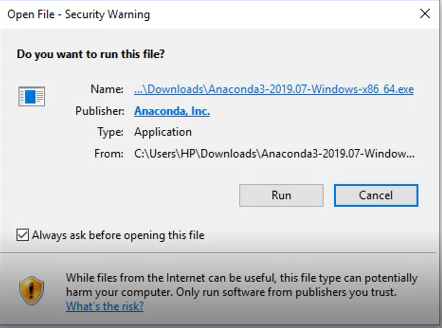
\includegraphics[scale=0.5]{figures/1}}
        \caption{Run Setup Anaconda}
		\label{langkah1}
\end{figure}

\item Tunggu hingga \textit{setup loading} selesai
\begin{figure}[H]
        \centerline{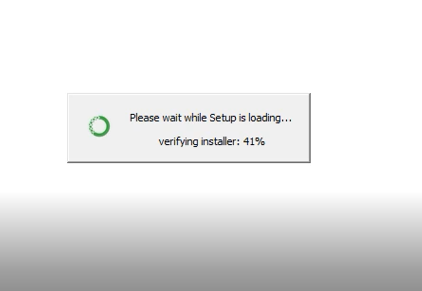
\includegraphics[scale=0.5]{figures/2}}
        \caption{Setup Loading}
		\label{langkah2}
\end{figure}


\item Jika \textit{setup loading} telah selesai, maka klik \textit{next}
\begin{figure}[H]
        \centerline{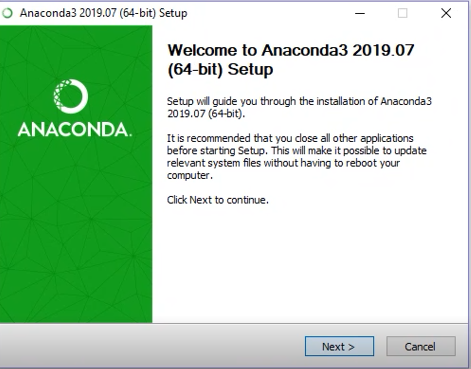
\includegraphics[scale=0.5]{figures/3}}
        \caption{Welcome to Anaconda Setup}
		\label{langkah2}
\end{figure}


\item Pada \textit{License Agreement} klik \textit{I Agree}
 gambar \textit{License Agreement}.

\begin{figure}[H]
    \centering
    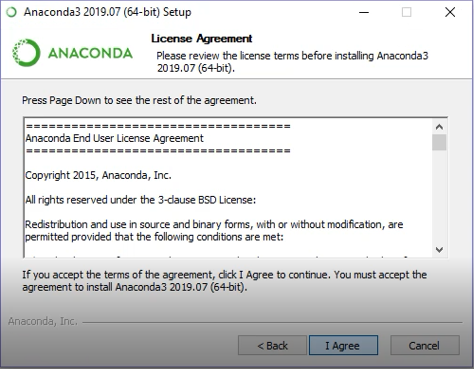
\includegraphics[scale=0.5]{figures/4}
    \caption{\textit{License Agreement}}
    \label{Figureanaconda3}
\end{figure}


\item Kemudian pilih \textit{Just Me(Recomended)} agar sesuai dengan komputer yang digunakan, kemudian klik \textit{next}
 gambar \textit{Just Me(recomended)}.

\begin{figure}[H]
    \centering
    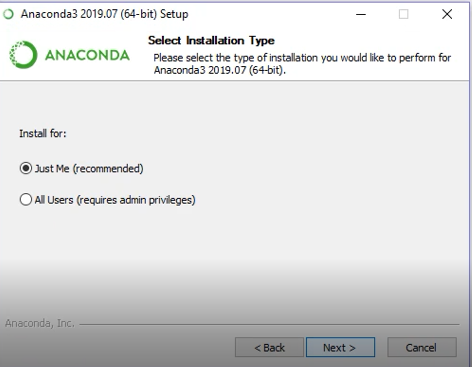
\includegraphics[scale=0.5]{figures/5}
    \caption{\textit{Just Me(recomended)}}
    \label{Figureanaconda4}
\end{figure}


\item Kemudian pilih lokasi tempat \textit{menginstall anaconda}
 gambar \textit{Pilih lokasi}.

\begin{figure}[H]
    \centering
    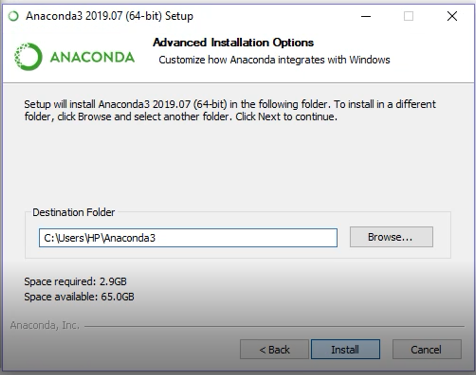
\includegraphics[scale=0.5]{figures/6}
    \caption{\textit{Pilih lokasi}}
    \label{Figureanaconda5}
\end{figure}

\item Kemudian centang \textit{Add Anaconda to my Path environtment variable}, agar saat \textit{menginstall selenium} langsung ke \textit{path anaconda} tidak ke aplikasi yang lain. Klik \textit{install}
 gambar \textit{Centang Anaconda to my PATH}.

\begin{figure}[H]
    \centering
    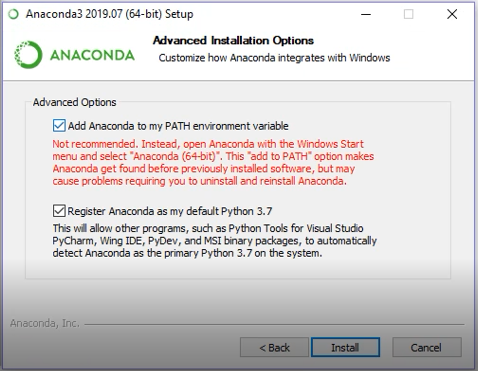
\includegraphics[scale=0.5]{figures/7}
    \caption{\textit{Centang Anaconda to my PATH}}
    \label{Figureanaconda6}
\end{figure}

\item Tunggu sampai proses \textit{installasi} selesai
 gambar \textit{Installation Complete}.

\begin{figure}[H]
    \centering
    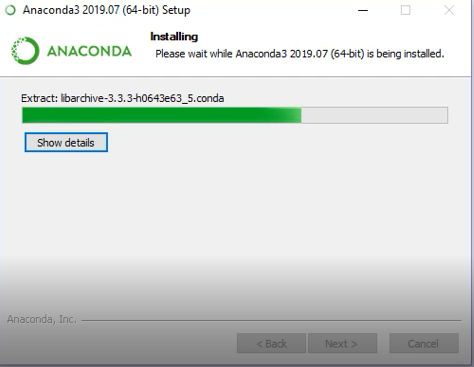
\includegraphics[scale=0.5]{figures/8}
    \caption{\textit{Installation Complete}}
    \label{Figureanaconda7}
\end{figure}

\item Apabila instalasi telah selesai klik \textit{next}
\begin{figure}[H]
    \centering
    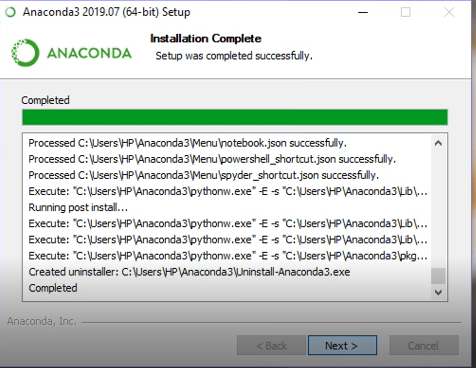
\includegraphics[scale=0.5]{figures/9}
    \caption{\textit{Installation Complete}}
    \label{Figureanaconda8}
\end{figure}

\item klik \textit{next}
\begin{figure}[H]
    \centering
    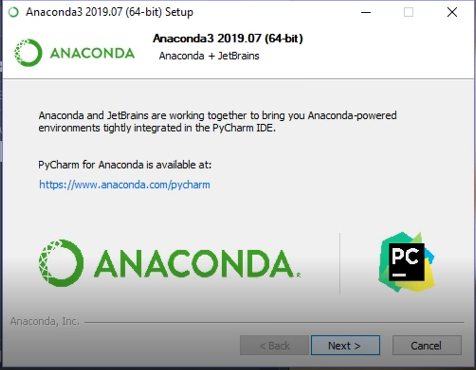
\includegraphics[scale=0.5]{figures/10}
    \caption{\textit{Anaconda+JetBrains}}
    \label{Figureanaconda70}
\end{figure}

\item Jika sudah klik \textit{finish}
 gambar \textit{Thanks fo install Anaconda}.

\begin{figure}[H]
    \centering
    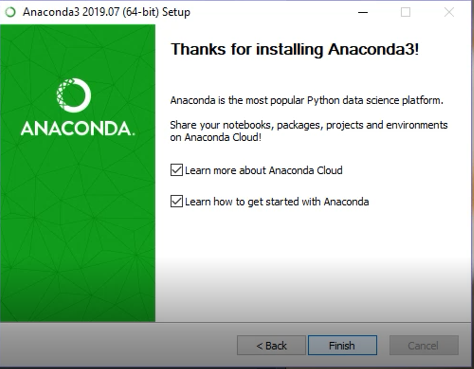
\includegraphics[scale=0.5]{figures/11}
    \caption{\textit{Thanks for install Anaconda}}
    \label{Figureanaconda70}
\end{figure}
\end{enumerate}

\section{Instalasi Pip}
\subsection{Windows (Windows 10)}
\begin{enumerate}
\item buka anaconda promt
\item ketikkan conda install -c anaconda pip
\begin{figure}[H]
    \centering
    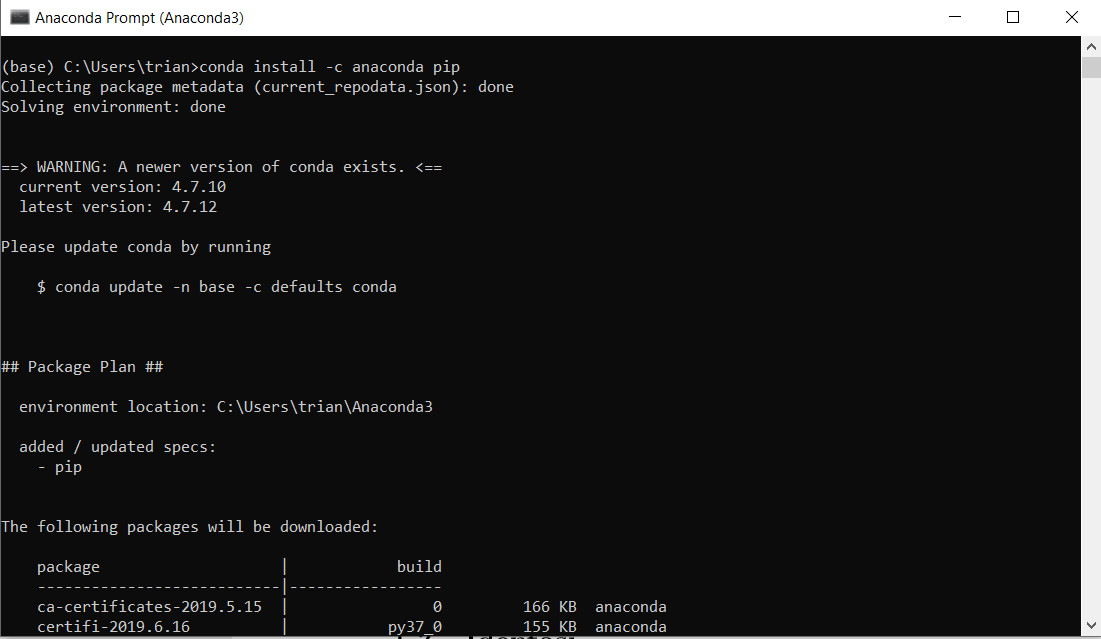
\includegraphics[scale=0.5]{figures/installpip (2)}
    \caption{\textit{Install pip}}
    \label{Figureanaconda70}
\end{figure}
\item ketik y, lalu enter. Tunggu hingga proses instalasi selesai.
\begin{figure}[H]
    \centering
    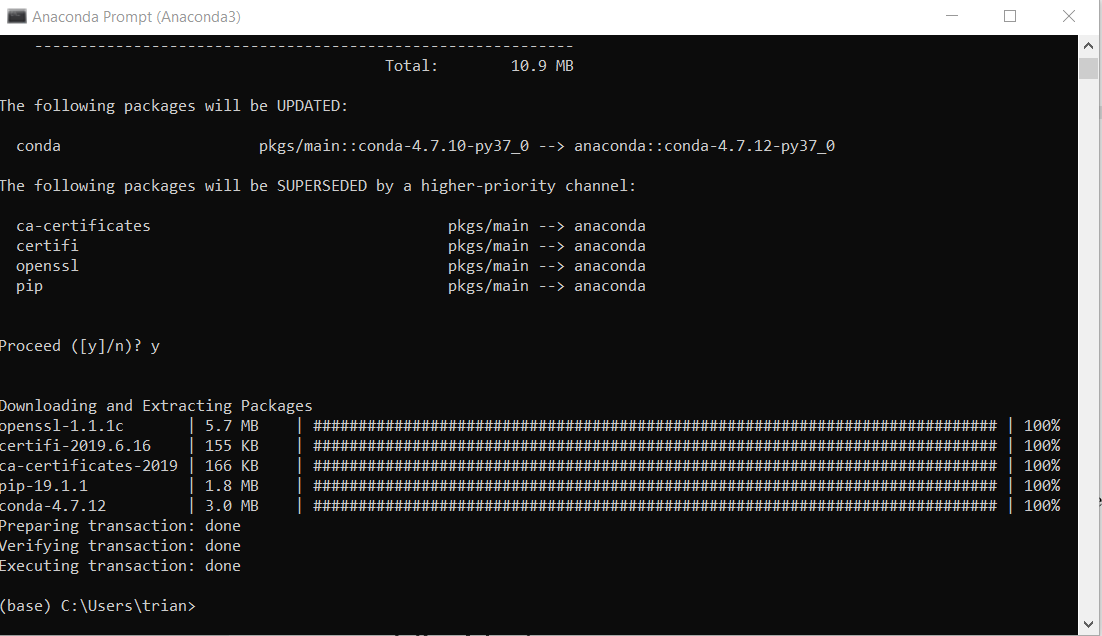
\includegraphics[scale=0.5]{figures/pipselesai}
    \caption{\textit{Install pip Selesai}}
    \label{Figureanaconda70}
\end{figure}
\item jika telah selesai, lakukan pengecekan versi pip dengan mengetikkan pip -V
\begin{figure}[H]
    \centering
    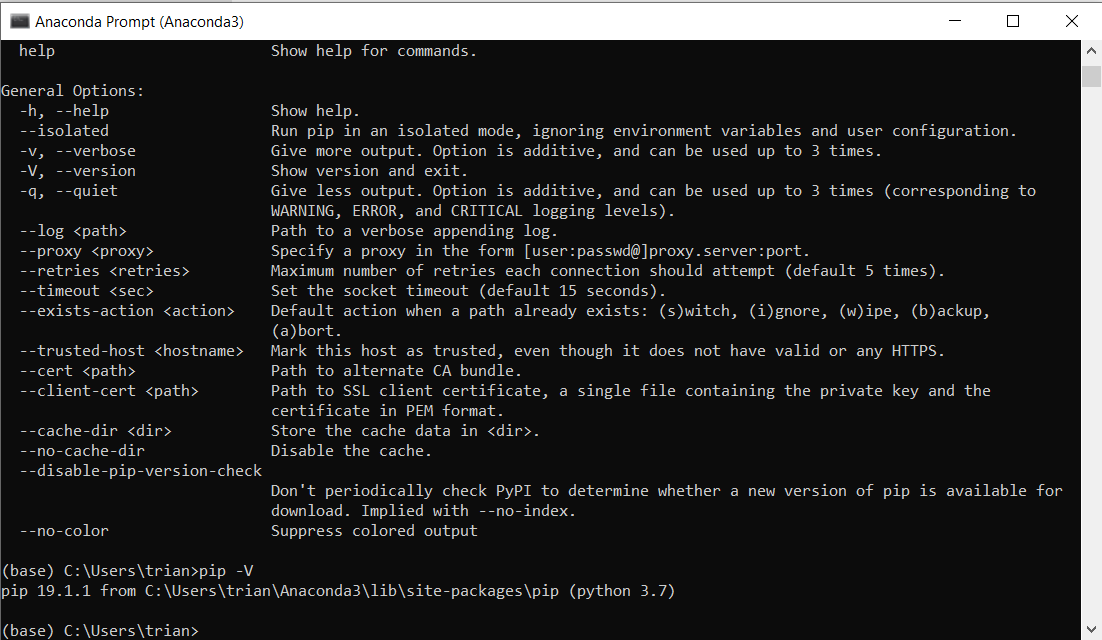
\includegraphics[scale=0.5]{figures/pipversion}
    \caption{\textit{Melihat Versi pip}}
    \label{Figureanaconda70}
\end{figure}

\end{enumerate}

\subsection{Linux (Ubuntu 19.04)}
\begin{enumerate}

\item pertama kita buka terminal kita lalu ketikkan perintah \textbf{sudo apt install python3-pip -y} untuk pip3 dan \textbf{sudo apt install python-pip -y} untuk pip contoh seperti gambar \ref{installpip}, lalu enter
\begin{figure}[H]
\centering
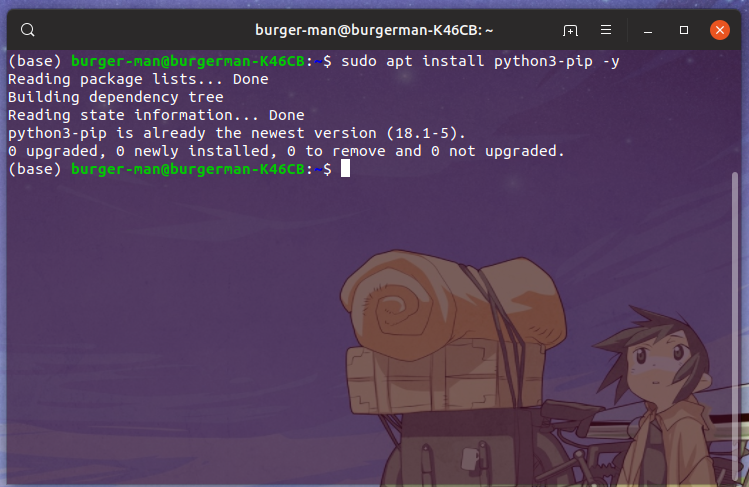
\includegraphics[width=1\textwidth]{figures/installpip.png}
\caption{Gambar instal pip}
\label{installpip}
\end{figure}

\end{enumerate}

\section{Setting Environment}
\subsection{Windows (Windows 10)}
\begin{enumerate}
\item Buka file explorer
\item Klik kanan pada This pc, lalu pilih properties
\begin{figure}[H]
    \centering
    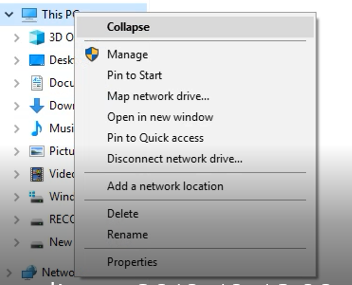
\includegraphics[scale=0.7]{figures/properties}
    \caption{\textit{Properties}}
    \label{Environment1}
\end{figure}
\item Pilih menu Advanced system settings
\begin{figure}[H]
    \centering
    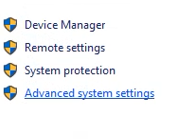
\includegraphics[scale=0.7]{figures/advanced}
    \caption{\textit{Advanced system settings}}
    \label{Environment2}
\end{figure}
\item Pilih Environment Variables
\begin{figure}[H]
    \centering
    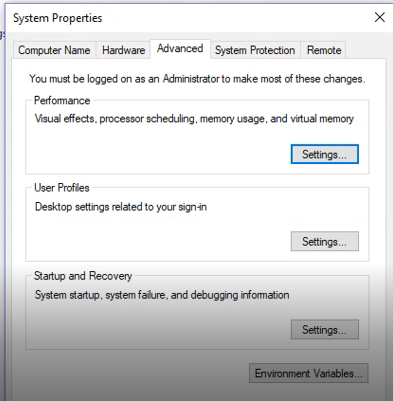
\includegraphics[scale=0.7]{figures/environment}
    \caption{\textit{Environment Variables}}
    \label{Environment3}
\end{figure}
\item Pilih Path
\begin{figure}[H]
    \centering
    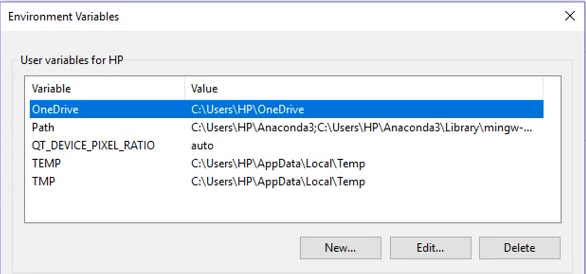
\includegraphics[scale=0.7]{figures/path}
    \caption{\textit{Path}}
    \label{Environment4}
\end{figure}
\item lalu pilih environment variable yang ingin ditambahkan, klik OK
\begin{figure}[H]
    \centering
    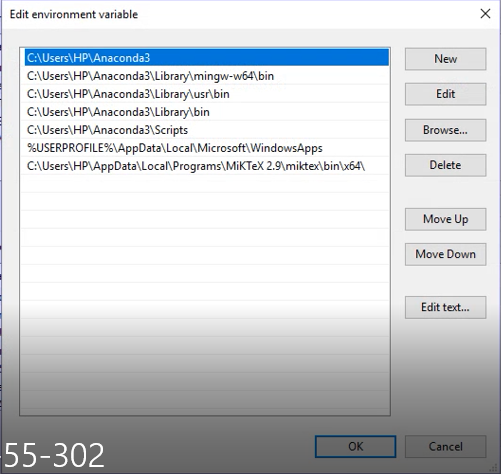
\includegraphics[scale=0.7]{figures/ok}
    \caption{\textit{Edit Environment Variable}}
    \label{Environment5}
\end{figure}
\end{enumerate}

\subsection{Linux (Ubuntu 19.04)}
\begin{enumerate}

\item pertama kita buka terminal kita lalu ketikkan perintah export PYTHONPATH=\$PYTHONPATH:pathinstallasipythonkalian contoh seperti gambar \ref{setpath}, lalu enter
\begin{figure}[H]
\centering
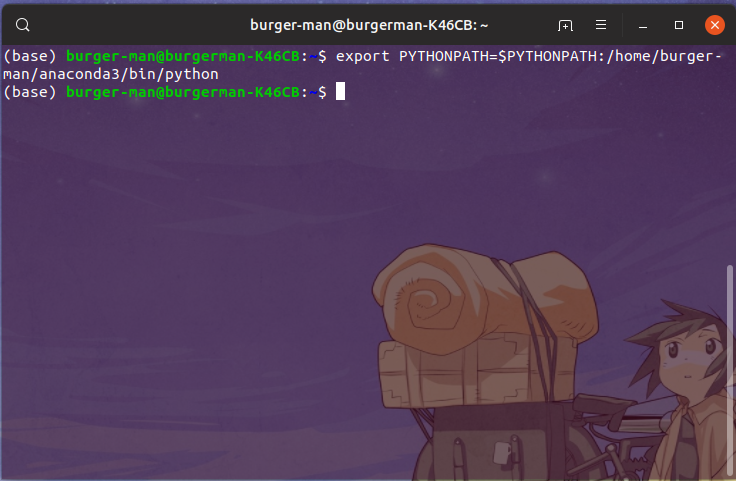
\includegraphics[width=1\textwidth]{figures/setpath.png}
\caption{Gambar setpath}
\label{setpath}
\end{figure}

\end{enumerate}

\section{Command Line Interface/Interpreter}
\subsection{Windows (Windows 10)}
\begin{enumerate}
\item Buka command prompt lalu ketikkan python
\item Buatlah perintah print, input, perkalian, dan pembagian
\item Bisa juga menjalankan file .py yang telah dibuat di IDE dengan cara python namafile.py, lalu klik enter
\begin{figure}[H]
    \centering
    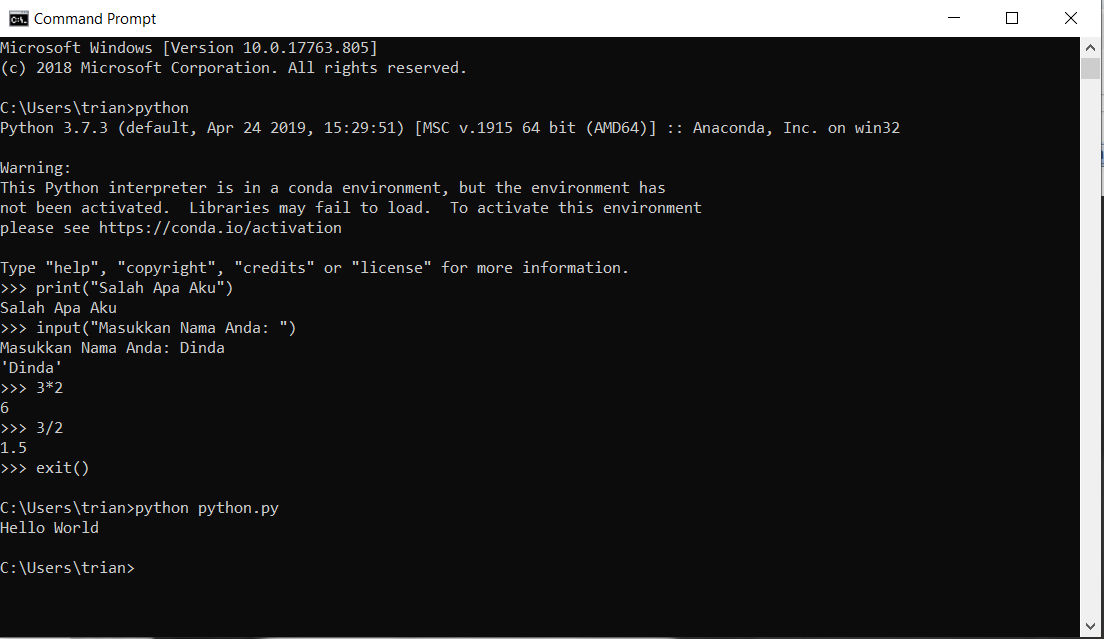
\includegraphics[scale=0.5]{figures/cli (2)}
    \caption{\textit{CLI in Command Prompt}}
    \label{CLI}
\end{figure}
\end{enumerate}

\subsection{Linux (Ubuntu 19.04)}
Untuk menjalankan perintah CLI cukup mudah yaitu sebagai berikut

\begin{enumerate}

\item Buka terminal lalu ketikkan \textbf{python \textit{namafile}.py} seperti gambar ~\ref{cli}, lalu enter
\begin{figure}[H]
\centering
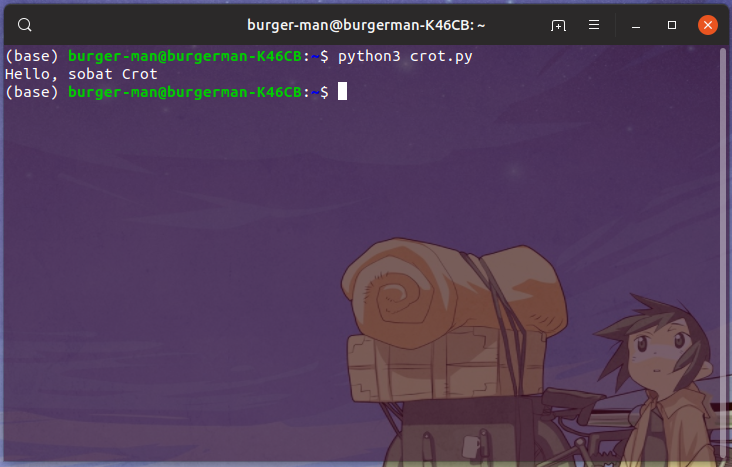
\includegraphics[width=1\textwidth]{figures/cli.png}
\caption{Gambar running script dengan CLI}
\label{cli}
\end{figure}

\end{enumerate}